\documentclass{article}
\usepackage{graphicx}

\begin{document}

\author{Eric Baucom}
\title{Automatic Syntactic Sentence Simplification with Transformation Based Learning: An Example}
\maketitle

In this short document, I will demonstrate a handful of fully worked example of syntactic sentence simplification within the Transformation-Based Learning (TBL) framework. Let us consider the following sentences, first the original ``complex'' sentence (after hand-curation) and then the simplified sentence:

\begin{quote}
In the 17th century the Empire was shattered by the Thirty Years' War.
\end{quote}

\begin{quote}
In the 17th century the Thirty Years' War shattered the Empire.
\end{quote}

In this example, we are dealing with the phenomenon of \textit{passive sentences}, one of three to be addressed in the thesis (the others being \textit{coordinate phrases} and \textit{quotative sentences}). The task of the simplification system will be to change the passive or ``complex'' sentence into its active or ``simplified'' equivalent.

The sentences will first be parsed using a constituency-based parser such as the Berkeley Parser. TBL relies on comparing the labels of tokens from the previous iteration of the algorithm to the current one. Candidate tokens will be collected by the longest matching substring algorithm. I will then make sure they are
constituent tokens using nltk's ``minimum spanning tree'' method, which gives the
tree position of the smallest subtree which dominates all and only a given
string of text. If a candidate token throws errors here, it may
indicate a parse error and could be useful in discussion and indicate
areas for further research (e.g., especially domain adaptation and other methods to improve parse quality). Many errors may indicate that a full
parse is the wrong level of analysis, and I may look into partial parsing or chunking.

\begin{figure}
\begin{center}
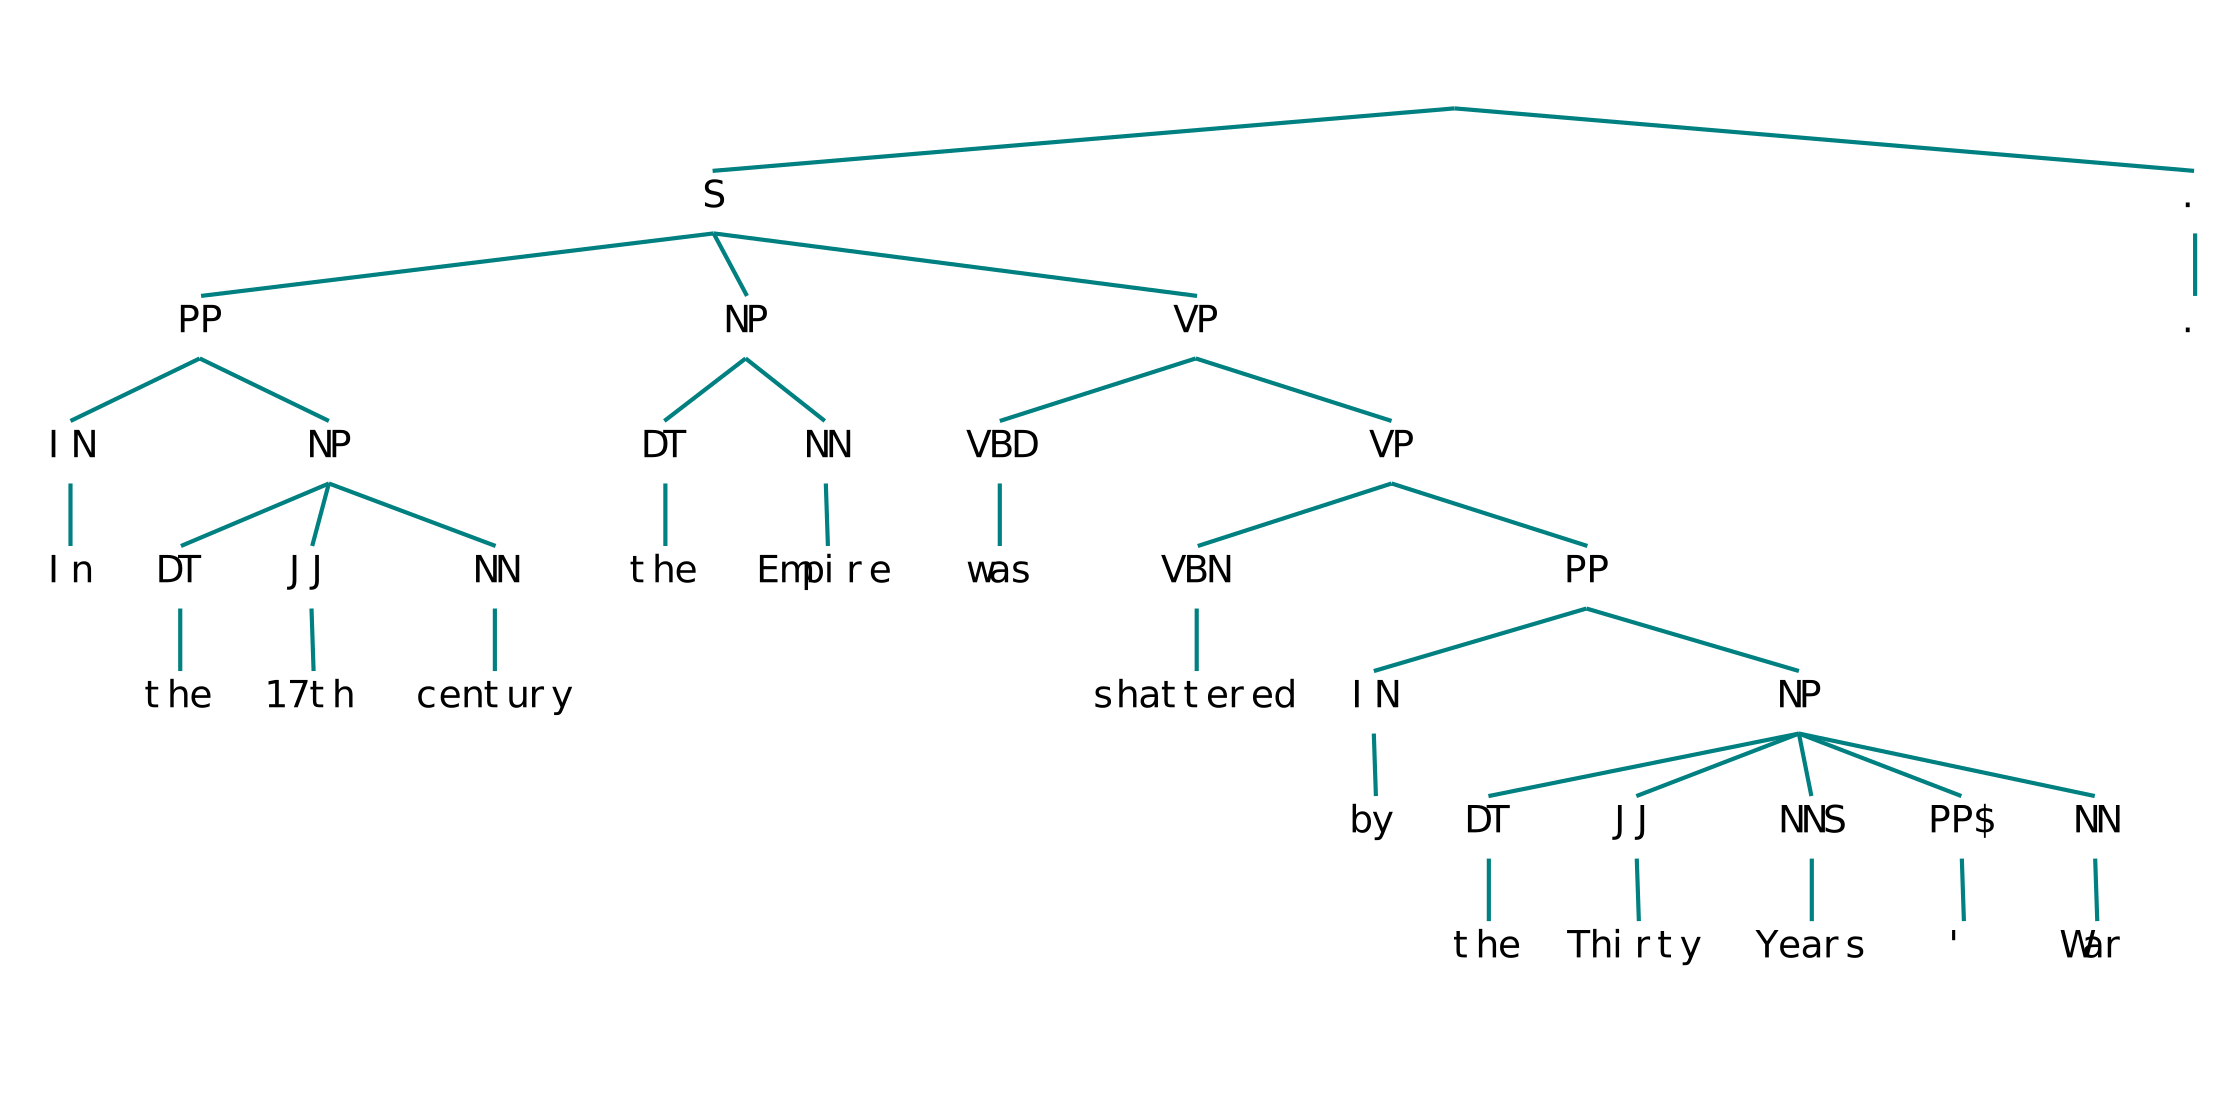
\includegraphics[scale=.65]{comp_pass}
\caption{The original complex passive sentence (after hand-curation).}
\end{center}
\end{figure}


\begin{figure}
\begin{center}
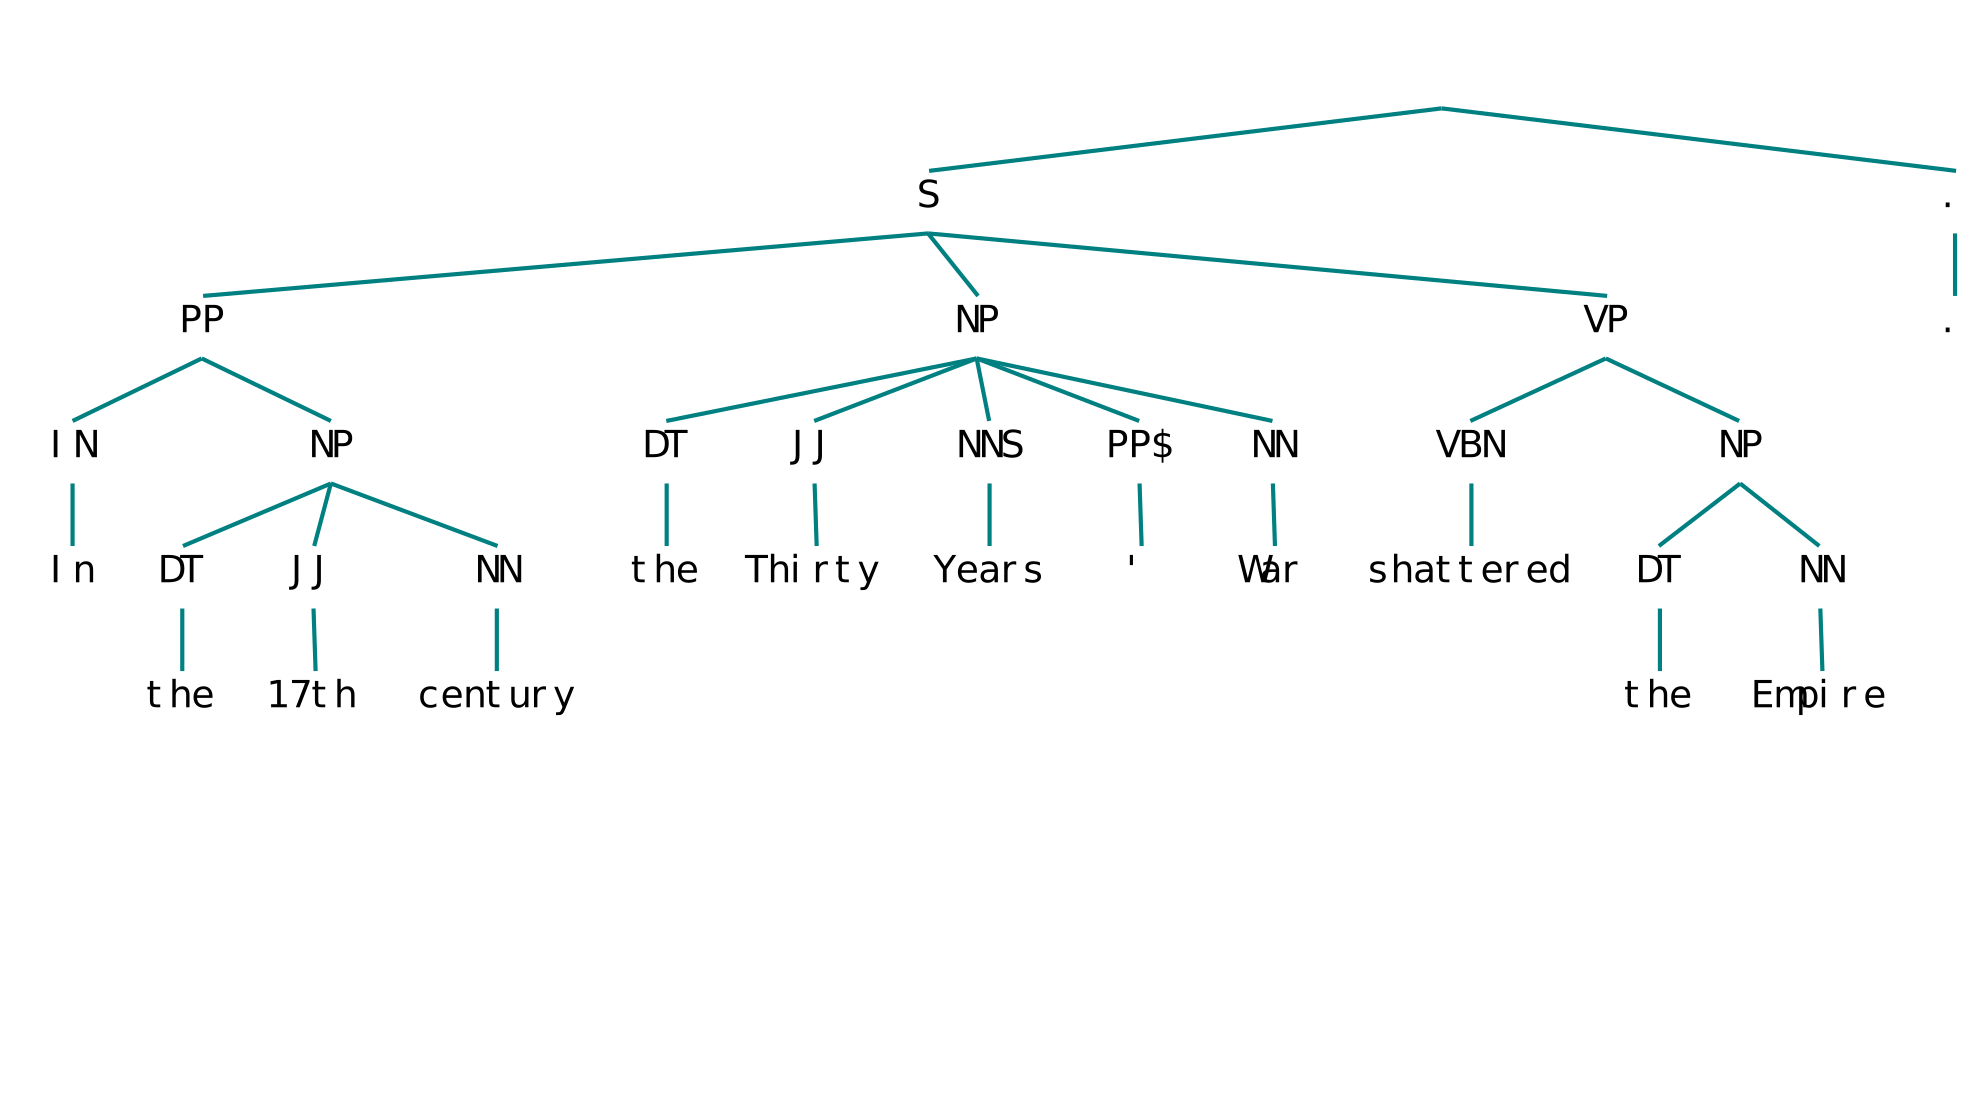
\includegraphics[scale=.65]{simp_pass}
\caption{The simplified active sentence.}
\end{center}
\end{figure}

Following this scheme, the following constituents will be extracted as being in common between the two sentences:

\begin{enumerate}
\item (\textbf{PP} \texttt{In the 17th century)}
\item (\textbf{NP} \texttt{the Empire)}
\item (\textbf{VBN} \texttt{shattered)}
\item (\textbf{NP} \texttt{the Thirty Years ' War)}
\item (\textbf{.} \texttt{.)}
\end{enumerate}

The constituents will then be assigned supertags in both the passive and active sentences which will correspond to their relative positions to the anchor of the sentence. The anchor will be the highest VP node of the sentence, which can be determined algorithmically via a breadth-first search. The highest VP is a useful anchor given its proximity to both the subject (typically left sibling) and the object(s) (typically the children to the right of the main verb child). The convention for supertags will be descriptive in relation to the anchor. The anchor will be represented by the character \texttt{a}. The descriptor \texttt{up} is used to indicate going to the parent of the current node. The other descriptors will be natural numbers indicating which child node to go to, in left-to-right linear order (it may prove to be useful to allow negative numbers indicating right-to-left linear order, which would mean two potential supertags for each token, but we will not discuss that further in this example). So, the supertag (a, 2, 3) would mean the constituent that is the anchor's second child's third child. See below for more examples.	

Notice that in the previous list, 1 and 5 maintain the same positions relative to the anchors of the two sentences, so they will be ignored as they present no ``errors'' to the TBL system (i.e., they have the same supertags in both sentences). The errors for the other consituents are shown below. The convention for errors in my implementation of TBL will be \textbf{\textless\textit{supertag-a}, \textit{supertag-b}, \textit{number-of-errors}\textgreater} (the number of errors is how TBL judges improvements between consecutive iterations).

\begin{enumerate}
\setcounter{enumi}{1}
\item \textbf{\textless(a,up,2), (a,2), 1\textgreater}
\item \textbf{\textless(a,2,1), (a,1), 1\textgreater}
\item \textbf{\textless(a,3,2), (a,up,2), 1\textgreater}
\end{enumerate}

We notice that \texttt{the Empire} has moved from the subject position to the object position. As mentioned, subjects are typically parsed as the left sibling of the anchor, and objects are typically the second child of the anchor. Notice that the subject in this case is not in the linear first position beside the anchor because of the preceding adjunct \texttt{In the 17th century}. So, we can generalize that the simplification process of passive sentences typically involves placing the subject in the object position. This can be represented by the following template:

\begin{center}
\textbf{Subj2Obj: (a,up,*) $\rightarrow$ (a,2)}
\end{center}

Here the asterisk can stand for any natural number. This template should generalize to most cases, including those with adjuncts before the original subject. The next case will be the main verb \textit{shattered}. It occurs originally in the canonical position, as the second child of the main VP after the passive \textit{(VBD was)}. And because of the minimum spanning tree algorithm, it is also the first and only child of its parent, giving \textbf{(a,2,1)}. This should almost always be the case for the location of the main verb in a passive sentence. Parsing a full corpus will tell otherwise, and adjustments will be made. But as of now the following template serves well and should generalize to many other sentences:

\begin{center}
\textbf{Pass2Act: (a,2,1) $\rightarrow$ (a,1)}
\end{center}

This places the verb in its proper spot as first child of the topmost VP. The last movement we have is the object of the preposition moving to the subject position. In this case we can be a bit more sophisticated with our template so as to generalize as much as possible. If the parent of the node is a PP and the linear-left sibling is \textit{(IN by)} we can deduce that this is the agent of the main verb and belongs in the subject position in the simplified sentence.

\begin{center}
\textbf{Agent2Subj-withAdjunct: (parent is PP, left-linear sibling is (IN by)) $\rightarrow$ (a,up,2)}
\end{center}

Note that this template only applies to sentences with a subject in second position after an adjunct. A corresponding template would have to be added to accomodate sentences without initial adjuncts.

So now if we imagine the algorithm at runtime, it would identify five tokens. It would identify the three errors and ignore cases that are not errors. Next, it would check for matching templates to correct the errors. \textbf{Subj2Obj} would run through each token (capping the number of possible siblings to 10 or 20) and would find a match, patching the first error. \textbf{Pass2Act} would trivially match and patch the error. \textbf{Agent2Subj-withAdjunct} would similarly run through each token and match and patch the correct error. The second iteration of the algorithm would reveal that no errors remain and would terminate.

The main challenge of the initial testing of the algorithm will be to create minimal and sufficient template lists that will cover the training data and generalize to the test data.

\begin{figure}
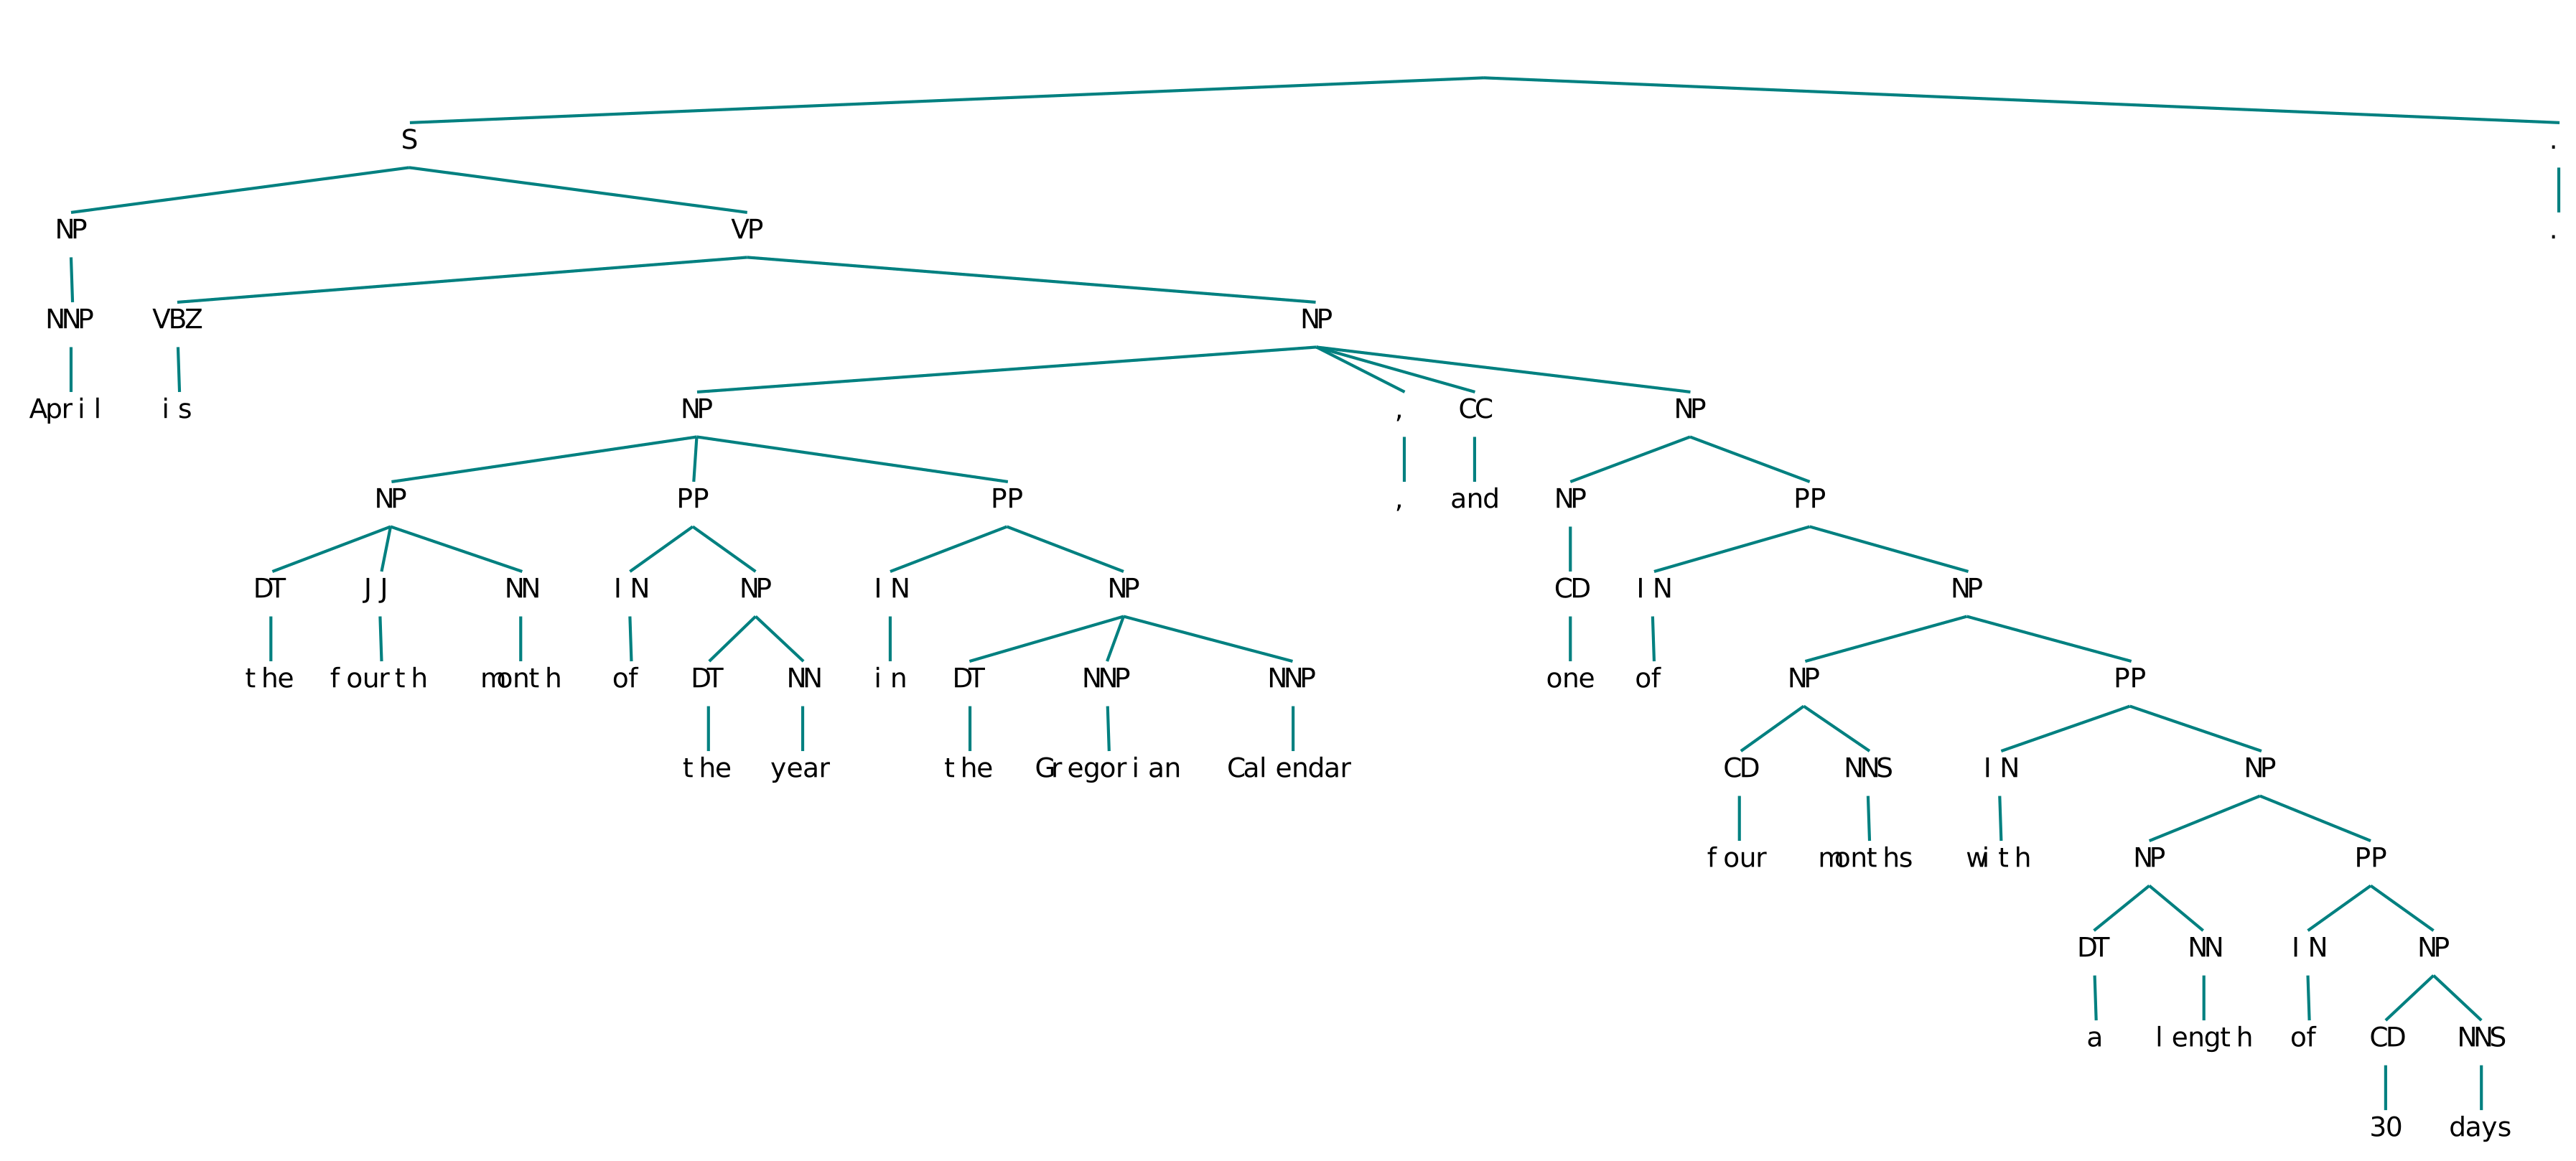
\includegraphics[scale=.45]{coord_tree}
\caption{The original complex coordinated sentence (after hand-curation).}
\end{figure}

\begin{figure}
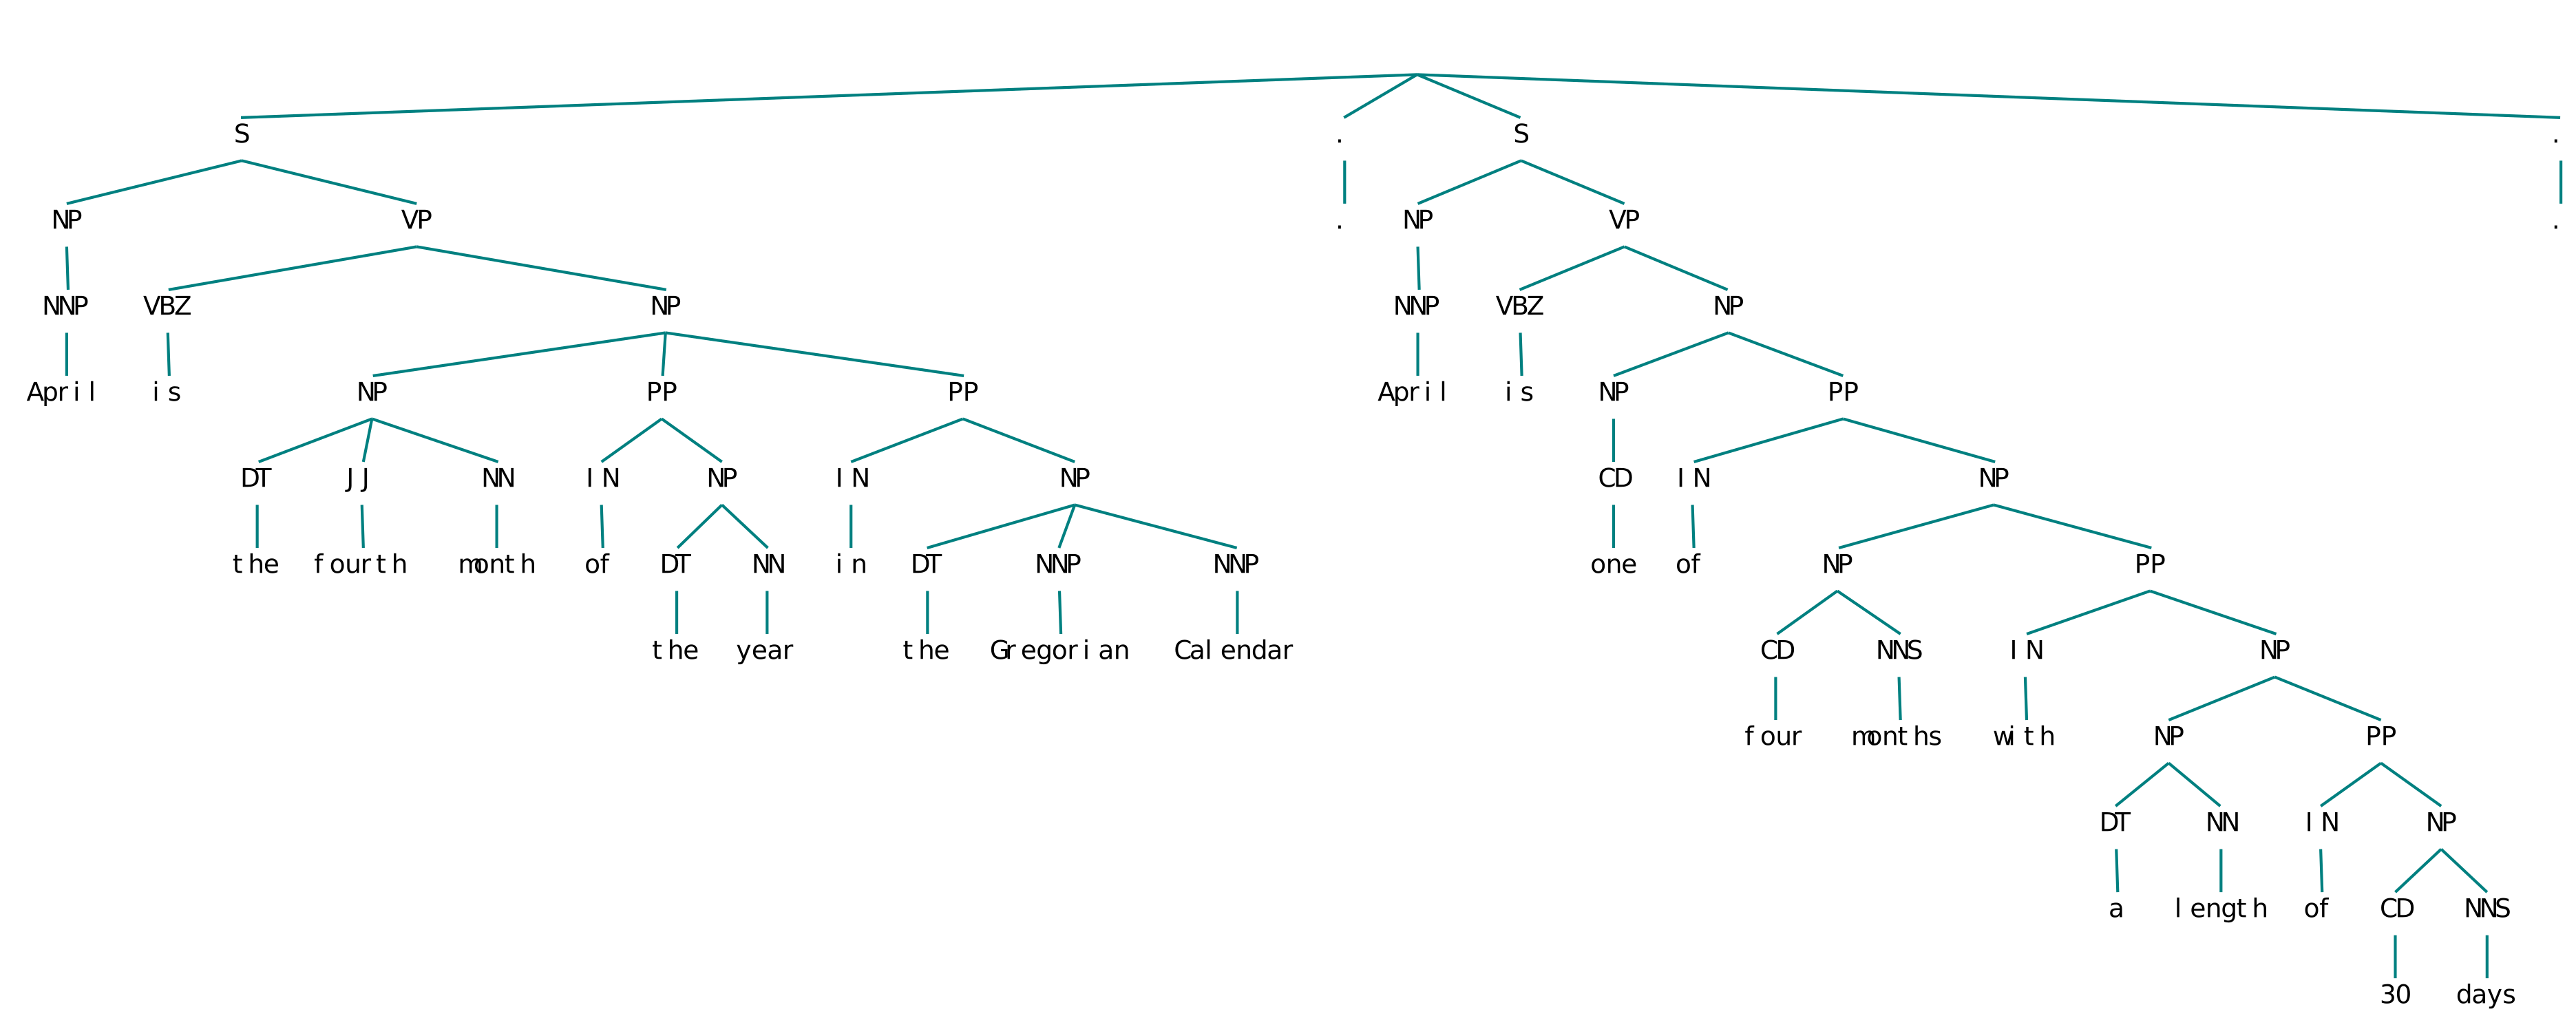
\includegraphics[scale=.41]{simp_coord}
\caption{The simplified ``de-coordinated'' sentence.}
\end{figure}

\begin{figure}
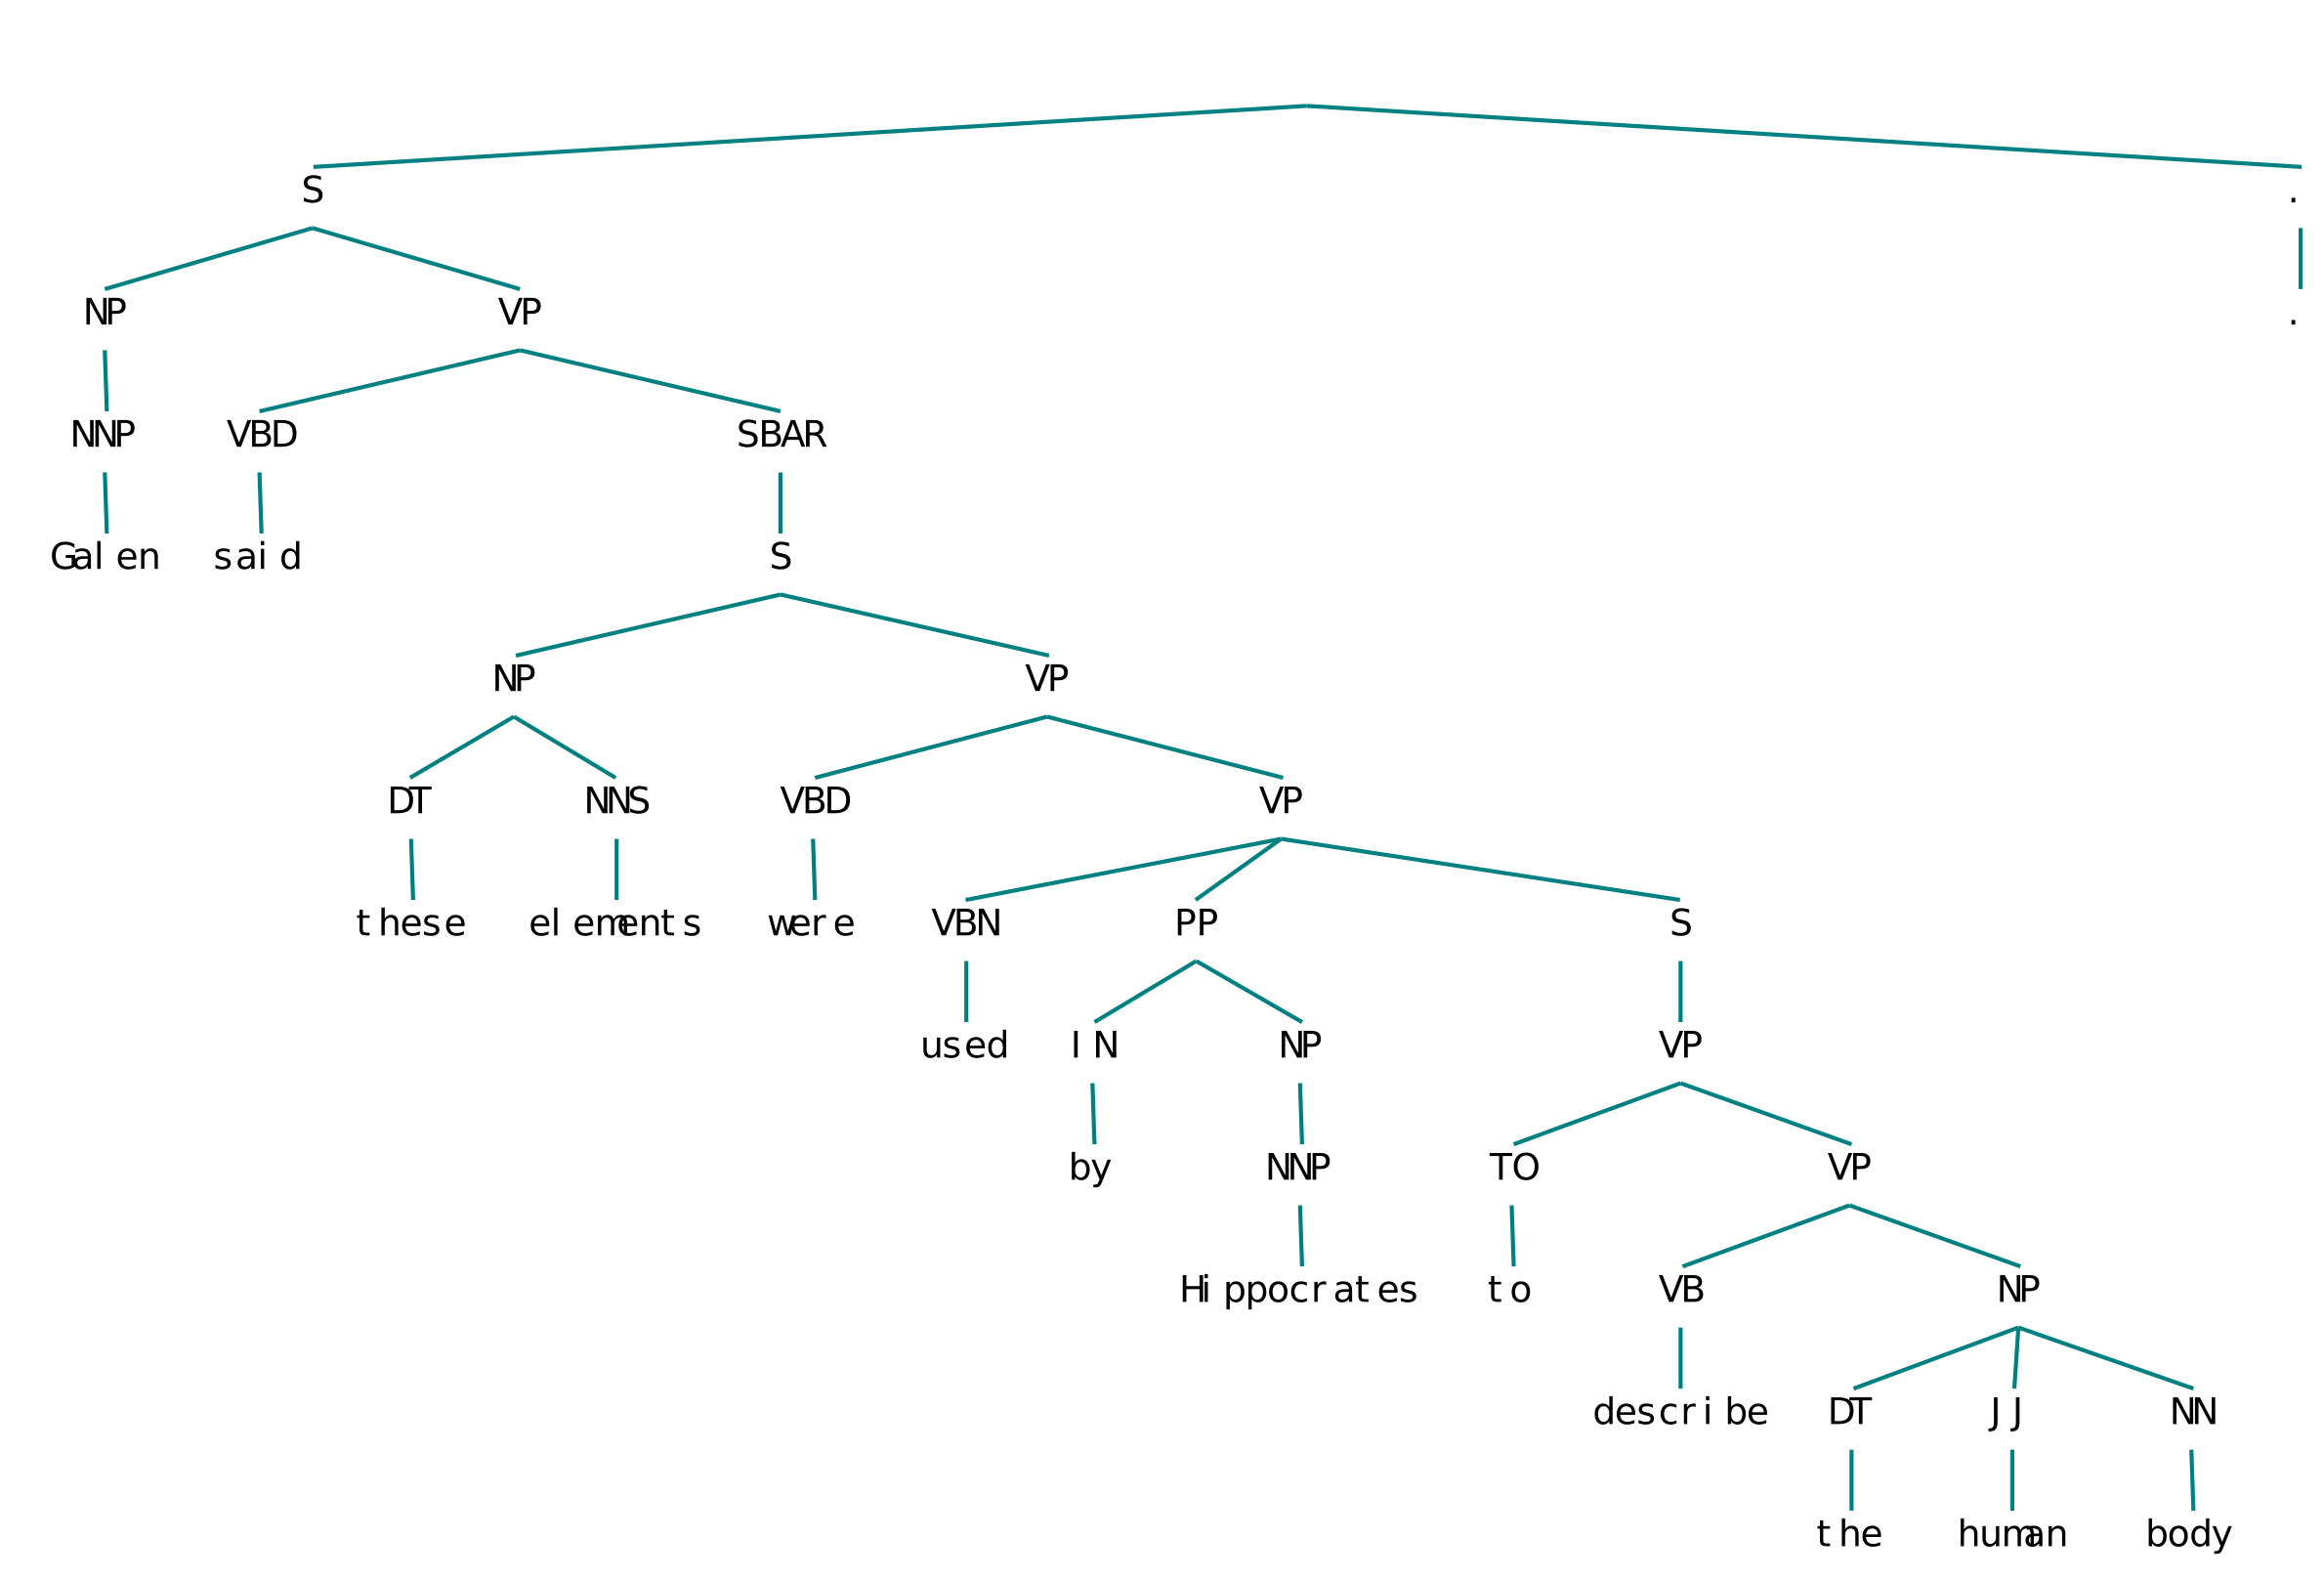
\includegraphics[scale=.6]{comp_quot}
\caption{The original complex reported sentence (after hand-curation).}
\end{figure}

\begin{figure}
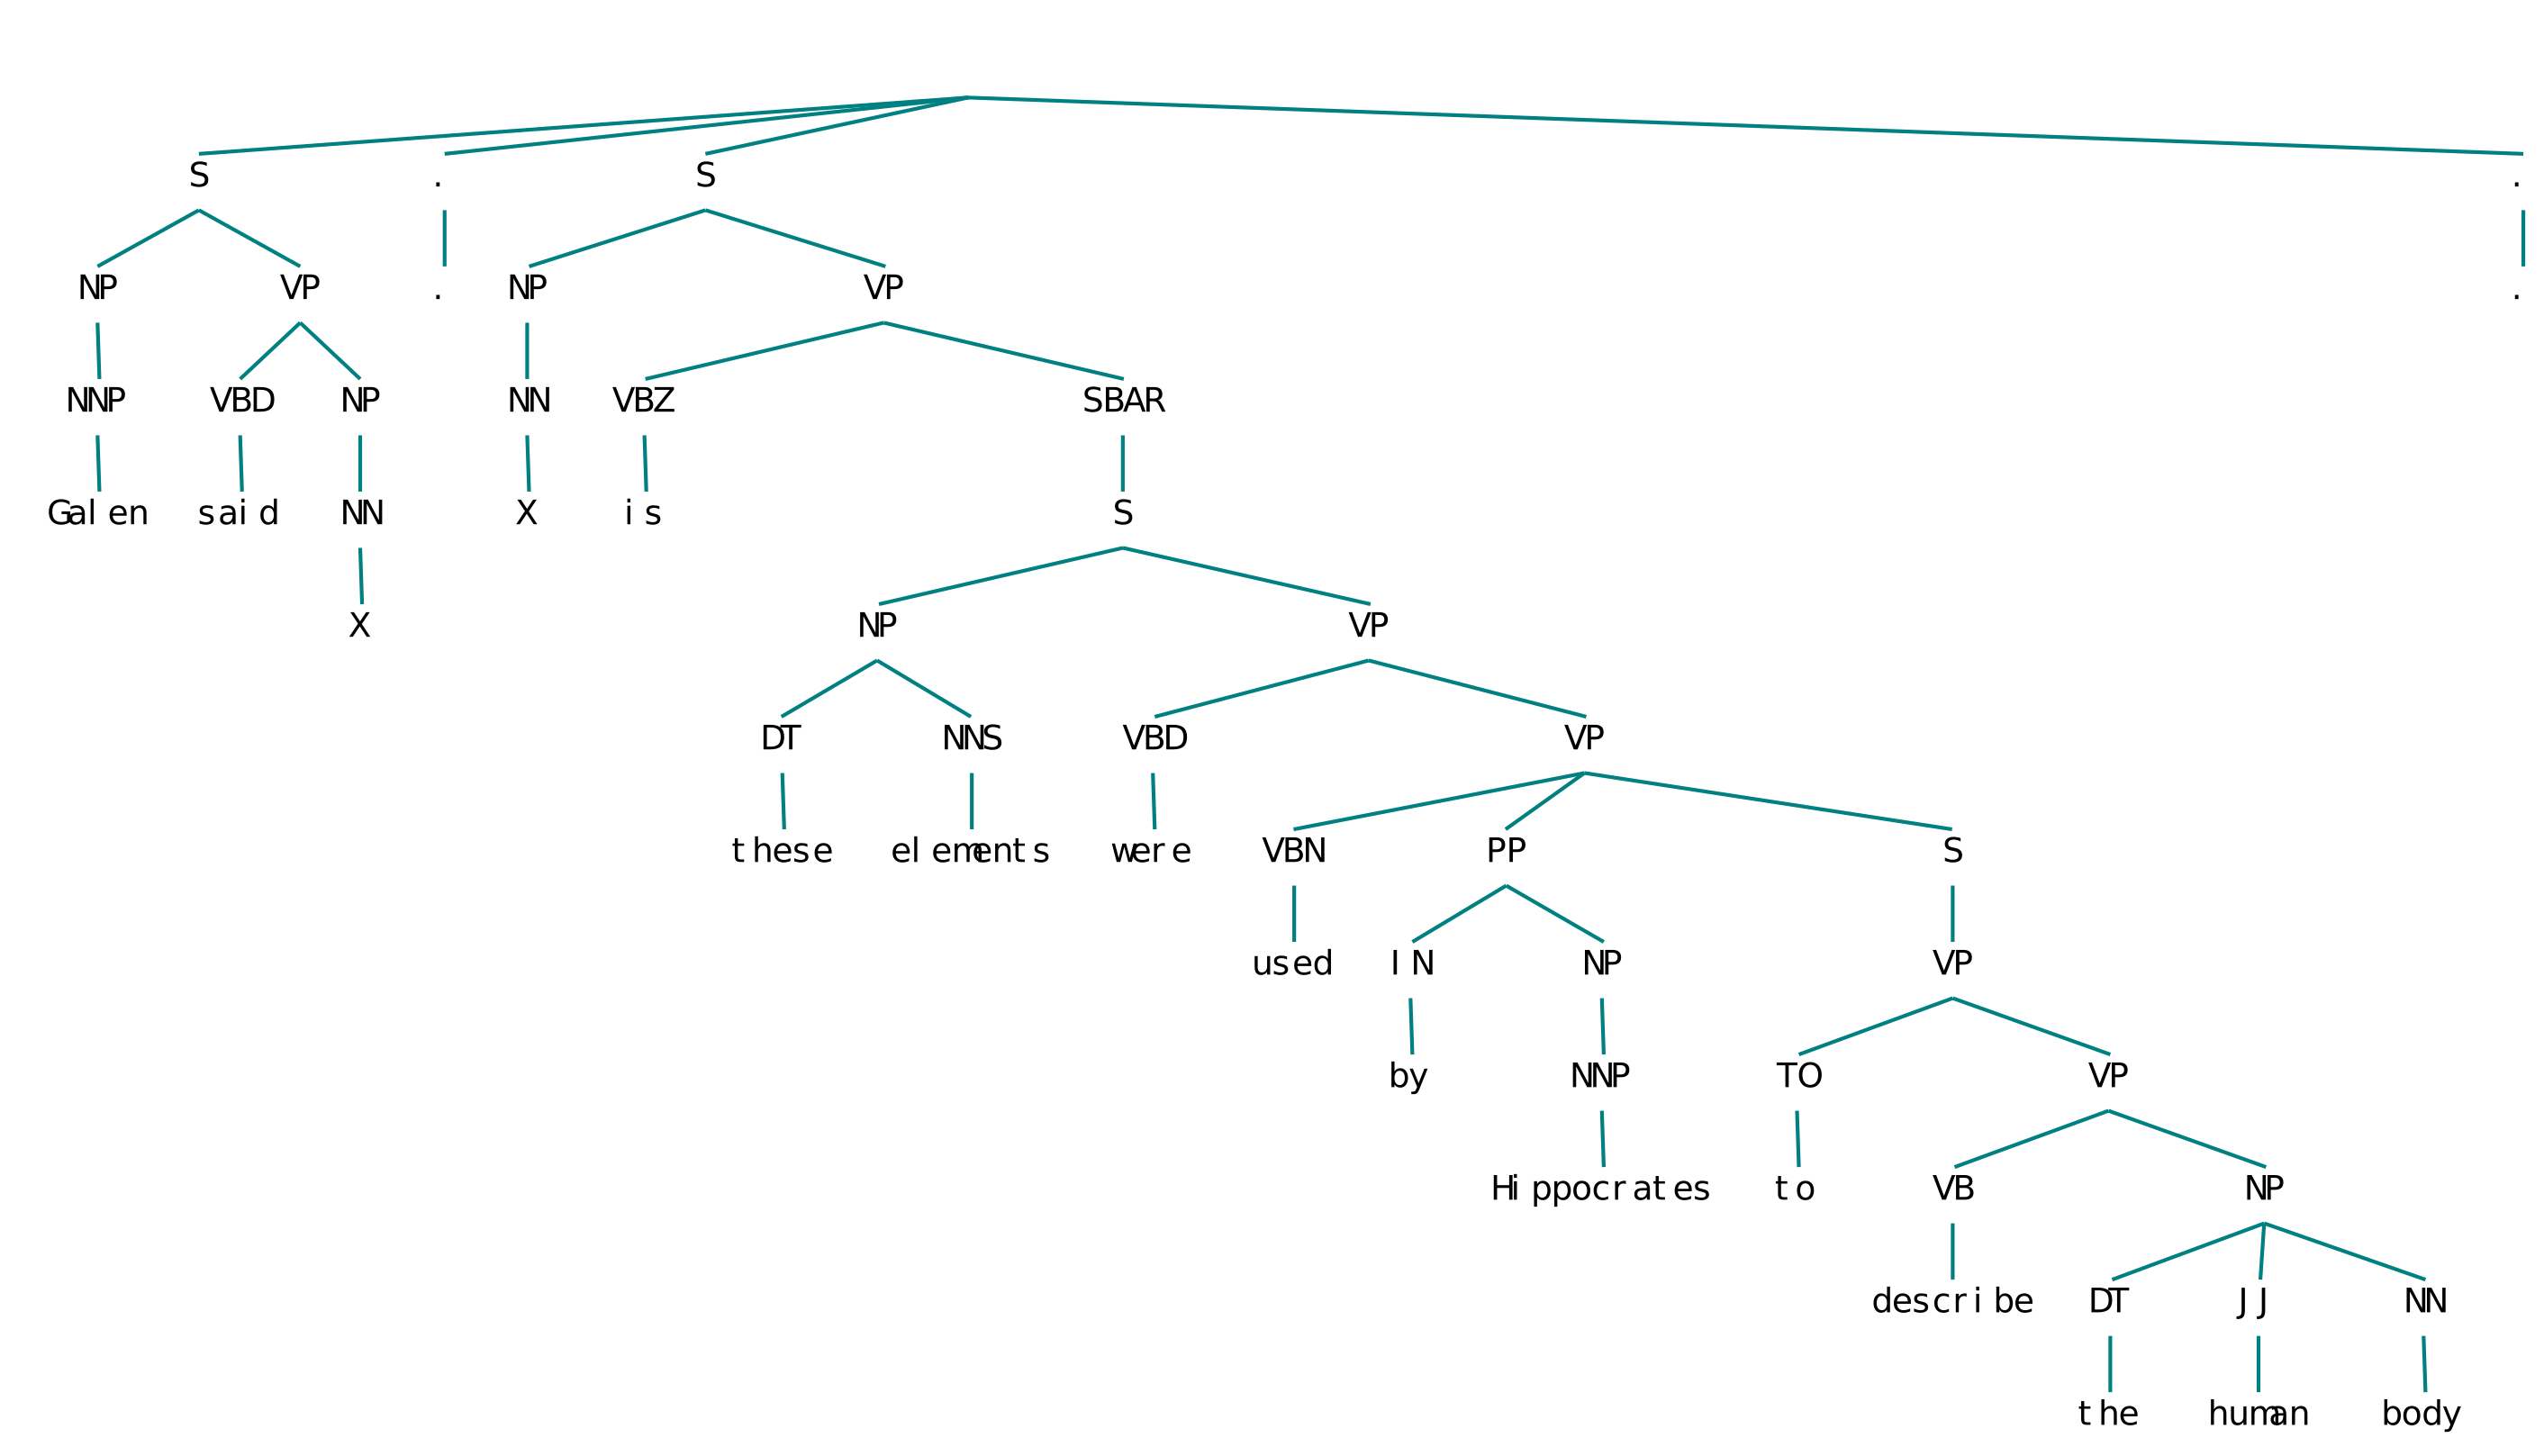
\includegraphics[scale=.56]{simp_quot}
\caption{The simplified reported sentence.}
\end{figure}


\end{document}